% Created 2022-04-02 Sat 14:56
% Intended LaTeX compiler: pdflatex
\documentclass[11pt]{article}
\usepackage[utf8]{inputenc}
\usepackage[T1]{fontenc}
\usepackage{graphicx}
\usepackage{grffile}
\usepackage{longtable}
\usepackage{wrapfig}
\usepackage{rotating}
\usepackage[normalem]{ulem}
\usepackage{amsmath}
\usepackage{textcomp}
\usepackage{amssymb}
\usepackage{capt-of}
\usepackage{hyperref}
\usepackage{tabularx}
\usepackage{minted}
\author{Adam Salwowski}
\date{\today}
\title{Statyczna strona portfolio wraz z poradnikami programistycznymi dla początkujących}
\hypersetup{
 pdfauthor={Adam Salwowski},
 pdftitle={Statyczna strona portfolio wraz z poradnikami programistycznymi dla początkujących},
 pdfkeywords={},
 pdfsubject={},
 pdfcreator={Emacs 27.1 (Org mode 9.3)}, 
 pdflang={Polish}}
\begin{document}

\maketitle
\tableofcontents


\section{Strona portfolio wraz z poradnikami programistycznymi dla początkujących}
\label{sec:orgfef9a19}
\subsection{Spis treści w języku polskim}
\label{sec:org41d7fad}
\subsection{Streszczenie w języku polskim}
\label{sec:org8fbd783}
\subsection{Spis treści w języku angielskim}
\label{sec:orgd57d9a0}
\subsection{Streszczenie w języku angielskim}
\label{sec:org7c2cd7a}
\subsection{Wstęp}
\label{sec:orgb914331}
Strona portfolio prezentująca projekty programisty. Centrum informacji dla początkujących programistów w postaci poradników i treściwych objaśnień.
\subsubsection{Cel projektu}
\label{sec:org86d683e}
\begin{enumerate}
\item Dla pracodawcy
\label{sec:orge224cf2}
\begin{itemize}
\item pokazanie z jakimi typami programista miał do czynienia
\item pokazanie sposobu rozwiązywania problemów
\item pokazanie jak wygląda kod (czy jest schludny i czytelny, lub może chaotyczny)
\item pokazanie czy dobrze zna technologie
\item pokazanie czy zna najnowsze rozwiązania w programowaniu
\end{itemize}
\item Dla programisty
\label{sec:orgc3b125f}
\begin{itemize}
\item pozwala uporządkować doświadczenie i przedstawić je lepiej niż w CV
\item pokazuje realne doświadczenie i wiedzę
\item pokazuje czego programista jeszcze nie robił i w jakim kierunku mógłby się jeszcze rozwinąć
\end{itemize}
\item Dla początkującego
\label{sec:org4f08aa9}
\begin{itemize}
\item miejsce w którym może się zapoznać w dość szybkim czasie z wieloma technologiami
\end{itemize}
\end{enumerate}
\subsubsection{Dla kogo ta aplikacja jest przeznaczona}
\label{sec:org92c1309}
\begin{itemize}
\item firmy zatrudniające programisów
\item początkujący programiści
\end{itemize}
\subsubsection{Użyte technologie użyte podczas produkcji strony}
\label{sec:org9955c1b}
\begin{itemize}
\item apache / nginx
\item html
\item css
\item org-mode
\item VPS (Virtual Private Server)
\item deployment strony
\item obraz png (zdjęcie)
\end{itemize}
\subsubsection{Użyte technologie podczas produkcji dokumentacji}
\label{sec:org8ad15ca}
\begin{itemize}
\item latex
\item org-mode
\end{itemize}
\subsubsection{Użyte technologie w celu dydaktycznym}
\label{sec:org2e2a2a5}
\begin{itemize}
\item instalacja niezbędnych pakietów
\item komendy unixowe:
\begin{itemize}
\item wget?
\item curl?
\item imagemagick?
\item ffmpeg?
\end{itemize}
\item konfiguracja środowiska programistycznego (edytor tekstowy Emacs)
\begin{itemize}
\item instalacja pakietów
\item przykładowe funkcje oraz ich działanie
\item obsługa magit?
\end{itemize}
\item python
\begin{itemize}
\item moduły:
\begin{enumerate}
\item argparse
\item pathlib
\item os
\item beautifulsoup4
\item requests
\end{enumerate}
\end{itemize}
\item html
\item css
\item java
\item c
\item c++
\item emacs lisp
\item latex
\item markdown
\item org-mode
\item regex
\item git
\end{itemize}
\subsection{Specyfikacja wymagań}
\label{sec:orgb5f07b0}
\subsubsection{{\bfseries\sffamily WORKING} Słownik pojęć}
\label{sec:org8011e52}
\subsubsection{specyfikacja grup użytkowników}
\label{sec:orgb595b09}
\subsubsection{pojęcia systemowe}
\label{sec:org9d61992}
\subsubsection{wymagania funkcjonalne}
\label{sec:org2d741fe}
dlaczego z jakiej strony, administator
\subsection{Użyte technologie}
\label{sec:org3a0cb69}
\subsubsection{opis używanych języków i technologii oprogramowania (html,css)}
\label{sec:org211c9b4}
\subsection{{\bfseries\sffamily TODO} Projekt aplikacji (UML) (zrobić na następne zajęcia!!!) (czy to w ogóle jest możliwe dla statycznej strony?, jeśli nie to poszukać dlaczego nie i napisac!!!!!)}
\label{sec:orgc15b29f}
\subsubsection{{\bfseries\sffamily DONE} Aktorzy}
\label{sec:org7bc48da}
\begin{description}
\item[{programista (ja)}] osoba odpowiedzialna za stworzenie strony
\item[{pracodawca}] osoba odpowiedzialna za zatrudnianie do firmy
\item[{początkujący}] osoba zaczynająca karierę w IT, ucząca się podstaw programowania
\end{description}
\subsubsection{{\bfseries\sffamily TODO} Diagram przypadków użycia}
\label{sec:org9cb336b}
\begin{enumerate}
\item {\bfseries\sffamily DONE} Przypadki użycia
\label{sec:orgaf42e03}
\begin{description}
\item[{strona}] cała strona z treścią dla \emph{początkujących} oraz \emph{pracodawców}
\item[{poradniki}] część strony wyznaczona dla \emph{początkującego}, zawierająca tutoriale
\item[{portfolio}] część strony wyznaczona dla \emph{pracodawcy}, zawierająca treści interesujące \emph{interviewerów} zatrudniających do firm
\item[{bibliografia / źródła}] treści które posłużyły \emph{programiście} przy budowie strony
\end{description}
\item {\bfseries\sffamily DONE} Funkcje
\label{sec:org0c9ce51}
\begin{description}
\item[{wyświetl stronę}] odpowiada za wyświetlenie strony za pomocą przeglądarki
\end{description}
\item {\bfseries\sffamily DONE} Diagramy
\label{sec:org6a3c625}

CLOSED: \textit{[2022-04-01 Fri 21:51]}
\begin{figure}[htbp]
\centering
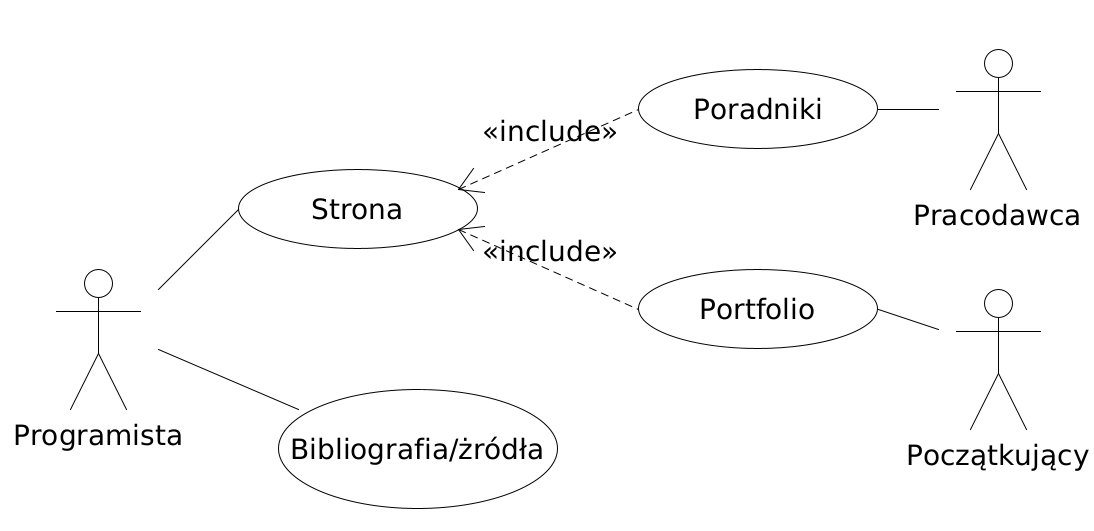
\includegraphics[width=.9\linewidth]{./images/diagram_przypadkow_uzycia.png}
\caption{Diagram przypadków użycia}
\end{figure}
\end{enumerate}
\subsubsection{{\bfseries\sffamily TODO} Diagram encji}
\label{sec:orgafbef7a}
\subsubsection{{\bfseries\sffamily TODO} Diagram klas}
\label{sec:org0e4607a}
\begin{enumerate}
\item Atrybuty klas
\label{sec:orgccc9222}
\begin{description}
\item[{Programista}] imie, nazwisko, e-mail, repozytoria, źródła
\item[{Początkujący}] imie, nazwisko, e-mail
\item[{Pracodawca/Interviewer}] imie, nazwisko, e-mail
\item[{Strona}] link, treść, technologie
\end{description}
\end{enumerate}

\subsection{Interfejs użytkownika}
\label{sec:orgc9678b8}
\subsubsection{Graficzna instrukcja użytkowania aplikacji}
\label{sec:org1f713c5}
\subsection{Podsumowanie efektu pracy}
\label{sec:org3ef8223}
\subsubsection{Jak można jeszcze rozwinąc aplikację w przyszłości}
\label{sec:orgea16a5b}
\subsubsection{Co się udało zrobić, a czego nie}
\label{sec:orgcbea82f}
\subsection{Bibliografia}
\label{sec:orgdee7b7e}
\subsubsection{Wykorzystane źródła}
\label{sec:orge04dfa3}
\begin{enumerate}
\item Kanały youtube?
\label{sec:org2b8a815}
\begin{itemize}
\item \url{https://youtube.com/channel/DistroTube}
\end{itemize}
\item Strony internetowe
\label{sec:orgd519135}
\begin{enumerate}
\item Strony portfolio
\label{sec:orga2f5ea4}
\begin{itemize}
\item \url{https://lukesmith.xyz}
\end{itemize}
\item Strony dydaktyczne
\label{sec:org9e92eaf}
\begin{itemize}
\item \url{https://landchad.net}
\item \url{https://xahlee.info}
\end{itemize}
\end{enumerate}
\item Książki
\label{sec:org21aaa9f}
\begin{itemize}
\item jakaś książka o emacs?
\item jakaś książka o
\end{itemize}
\item Prezentacje?
\label{sec:org0f6be42}
\end{enumerate}
\subsubsection{nie tylko strony internetowy, mają być książki, prezentacje}
\label{sec:orgd2344b3}
\subsection{Podsumowanie}
\label{sec:org4056448}
\end{document}